\documentclass[12pt,a4paper]{article}

\usepackage[left=3.00cm, right=2.00cm, top=2.00cm, bottom=2.00cm]{geometry}
\usepackage{lmodern}
\usepackage[T1]{fontenc}
\usepackage[utf8]{inputenc}
\usepackage[brazil]{babel}
\usepackage{microtype}

\usepackage{indentfirst,setspace}
\setlength{\parindent}{1.3cm}
\setlength{\parskip}{0.2cm}
\singlespacing

\usepackage{amssymb,amsmath,amsfonts}

\usepackage[numbers]{natbib}
\usepackage{url}
\bibliographystyle{plainnat}

\usepackage{longtable}
\usepackage{booktabs}
\usepackage[skip=1pt,labelfont=bf]{caption}
\usepackage{float}

\usepackage{array}

\usepackage{graphicx}
\graphicspath{ {./imgs/} }

\numberwithin{figure}{subsection}
\numberwithin{table}{subsection}

\usepackage{lipsum}

\author{Pablo Cecilio Oliveira\\
Marcilene Reis}
\title{Primeiro Trabalho Prático de AOC I\\
Assembly MIPS}
\date{}

\begin{document}
\maketitle

\section{Introdução}

Mambojambo introduzindo sobre o que é o documento, as questões, Mars, etc.

\lipsum[1]

\section{Implementação}

\subsection{Questão 1}

O procedimento para calcular o $cosseno$ de um ângulo segundo a série de Taylor abaixo:
\[ \cos x = \sum_{n=0}^{\infty} \frac{(-1)^n}{(2n)!} x^{2n} \]

A função $seno$ chama funções para calcular o fatorial e a função potência de $x$. O usuário digita o ângulo em radianos e a quantidade de termos da série ($n>0$).

\subsection{Questão 2}

O programa lê uma \texttt{string} de um arquivo denominado \texttt{entrada.txt} e gera um novo arquivo de nome \texttt{saida.txt} contendo uma nova \texttt{string} processada. 

A \texttt{string} gerada no arquivo de saída possui seus caracteres maiúsculos trocados por minúsculos, e seus  caracteres minúsculos trocados por maiúsculos.

Para iniciar o processamento, inicialmente os dados dos arquivos a serem carregados são declarados, assim como é definido o espaço reservado para o buffer de leitura do arquivo de entrada.

\begin{table}[H]
	\begin{tabular}{>{\ttfamily}l>{\ttfamily}l}
	.data   & \\
	fin:	& .asciiz "entrada.txt" \\
	fout:	& .asciiz "saida.txt" \\
	string:	& .space 1024 \\
	\end{tabular}
\end{table}

Inicia .text. A chamada para os procedimentos e a passagem das referencias.

\begin{table}[H]
	\renewcommand{\arraystretch}{1}
	\centering
	\caption*{Escopo principal do programa}
	\label{q2cod:main}
	\begin{tabular}{>{\ttfamily}p{4cm} p{11cm}}
		\toprule
		main:              & \\
		\midrule
		la \$a0,fin	       & atribui o arquivo de entrada a \ttfamily{\$a0} \\
		jal leArquivo      & inicia o procedimento \\
		la \$a0,string     & atribui a string a \ttfamily{\$a0} \\
		jal manipulaString & inicia o procedimento \\
		la \$a0,fout       & atribui o arquivo de saida a \ttfamily{\$a0} \\
		jal salvaArquivo   & inicia o procedimento \\
		li \$v0,10         & system call: Saia do programa \\
		syscall            & Saia! \\
		\bottomrule
	\end{tabular}
\end{table}

Procedimento \texttt{leArquivo} mais comentários a respeito de seu funcionamento por etapas e breve sumario de conclusão desse.

\begin{table}[H]
	\renewcommand{\arraystretch}{1}
	\centering
	\caption*{Procedimento para ler o arquivo}
	\label{q2cod:lefile}
	\begin{tabular}{>{\ttfamily}p{4cm} p{11cm}}
		\toprule
		leArquivo:       & \\
		\midrule[0.01cm]
		li \$v0,13       & system call: Abre o arquivo \\
		li \$a1,0        & flag para somente leitura \\
		li \$a2,0        & modo ignorado \\
		syscall          & Abra o arquivo! \\
		move \$t0,\$v0   & Salva o descriptor em \ttfamily{\$t0} \\
		\midrule[0.01cm]
		li \$v0,14       & system call: Lendo o arquivo \\
		move \$a0,\$t0   & Carrega o descriptor do arquivo \\
		la \$a1,string   & endereco do buffer \\
		li \$a2,255      & hardcoded buffer length \\
		syscall          & Leia o arquivo! \\
		move \$s0,\$v0   & Salva strlen em \ttfamily{\$s0} \\
		\midrule[0.01cm]
		li \$v0,16       & system call: Fecha o arquivo \\
		syscall          & Feche o arquivo! \\
		\midrule[0.01cm]
		jr \$ra          & Retorna do procediemnto \\
		\bottomrule
	\end{tabular}
\end{table}

Procedimento \texttt{manipulaString} mais comentários a respeito de seu funcionamento por etapas e breve sumario de conclusão desse.

\lipsum[1]

\begin{table}[H]
	\renewcommand{\arraystretch}{1}
	\centering
	\caption{Tabela ASCII para A-Z e a-z}
	\label{tab:ascii}
	\begin{tabular}{rl|rl|rl|rl|rl|rl|rl}
		\toprule
		 65 & A &  69 & E &  73 & I &  77 & M &  81 & Q &  85 & U &  89 & Y \\
		 66 & B &  70 & F &  74 & J &  78 & N &  82 & R &  86 & V &  90 & Z \\
		 67 & C &  71 & G &  75 & K &  79 & O &  83 & S &  87 & W &     &   \\
		 68 & D &  72 & H &  76 & L &  80 & P &  84 & T &  88 & X &     &   \\
		\midrule
		 97 & a & 101 & e & 105 & i & 109 & m & 113 & q & 117 & u & 121 & y \\
		 98 & b & 102 & f & 106 & j & 110 & n & 114 & r & 118 & v & 122 & z \\
		 99 & c & 103 & g & 107 & k & 111 & o & 115 & s & 119 & w &     &   \\
		100 & d & 104 & h & 108 & l & 112 & p & 116 & t & 120 & x &     &   \\
		\bottomrule
		\multicolumn{12}{l}{\footnotesize Fonte: \citet*{wiki:xxx}}
	\end{tabular}
\end{table}

\begin{table}[H]
	\renewcommand{\arraystretch}{1}
	\centering
	\caption*{Procedimento para alterar a string}
	\label{q2cod:manipula}
	\begin{tabular}{>{\ttfamily}p{5cm} p{10cm}}
		\toprule
		manipulaString:        & \\
		\midrule[0.01cm]
		Loop:                  & loop para cada caractere da string \\
		lb \$t2,(\$a0)         & Aponta \$t2 para a posição de endereço de \ttfamily{\$a0} \\
		beq \$t2,\$zero,End    & Se \$t2 conter NULL, a string terminou, \ttfamily{End} \\
		slti \$t1,\$t2,90      & \$t2 e menor que 90(Z)? \\
		bne \$t1,\$zero,Upper  & Se \$t1 for 1 então 1 != 0, vai pra \ttfamily{Upper} \\
		slti \$t1,\$t2,122     & \$t2 e menor que 122(z)? \\
		bne \$t1,\$zero,Lower  & Se \$t1 for 1 então 1 != 0, vai pra \ttfamily{Lower} \\
		j Next                 & Va pra Next \\
		\midrule[0.01cm]
		Upper:                 & rotina para uppercase \\
		slti \$t1,\$t2,65      & \$t2 e menor que 65(A)? \\
		bne \$t1,\$zero,Next   & Se \$t1 for 1 então não é uma letra, \ttfamily{Next} \\
		addi \$t2,\$t2,32      & Soma 32 a \$t2 \\
		sb \$t2,(\$a0)         & armazena o valor na posição em \ttfamily{\$a0} \\
		j Next                 & Va pra Next \\
		\midrule[0.01cm]
		Lower:                 & rotina para lowercase \\
		slti \$t1,\$t2,97      & \$t2 e menor que 97(a)? \\
		bne \$t1,\$zero,Next   & Se \$t1 for 1 então não é uma letra, Next \\
		addi \$t2,\$t2,-32     & Soma -32 a \ttfamily{\$t2} \\
		sb \$t2,(\$a0)         & armazena o valor na posição em \ttfamily{\$a0} \\
		\midrule[0.01cm]
		Next:                  & Continua a interação \\
		addi \$a0,\$a0,1       & Incrementa o endereço de \ttfamily{\$a0} \\
		j Loop                 & Va para Loop \\
		\midrule[0.01cm]
		End:                   & Termino do Loop \\
		jr \$ra                & Retorna do procedimento \\
		\bottomrule
	\end{tabular}
\end{table}

Procedimento \texttt{salvaArquivo} mais comentários a respeito de seu funcionamento por etapas e breve sumario de conclusão desse.

\begin{table}[H]
	\renewcommand{\arraystretch}{1}
	\centering
	\caption*{Procedimento para salvar o arquivo}
	\label{q2cod:salvafile}
	\begin{tabular}{>{\ttfamily}p{4cm} p{11cm}}
		\toprule
		salvaArquivo:    & \\
		li \$v0, 13      & system call: Abre o arquivo \\
		li \$a1, 1       & flag para escrita \\
		li \$a2, 0       & modo ignorado \\
		syscall          & Abra o arquivo! \\
		move \$t0,\$v0   & Salva o descriptor em \$t0 \\
		\midrule[0.01cm]
		li \$v0,15       & system call: Escrevendo no arquivo \\
		move \$a0,\$t0   & Carrega o descriptor do arquivo \\
		la \$a1,string   & endereço do buffer \\
		move \$a2,\$s0   & carrega strlen de \$s0 \\
		syscall          & Escreva no arquivo! \\
		\midrule[0.01cm]
		li \$v0,16       & system call: Fecha o arquivo \\
		syscall          & Feche o arquivo! \\
		jr \$ra          & Retorna do procedimento \\
		\bottomrule
	\end{tabular}
\end{table}

\lipsum[1]

\begin{figure}[H]
	\centering
	\caption{Questão 2, estatísticas das instruções.}
	\vspace{0.2cm}
	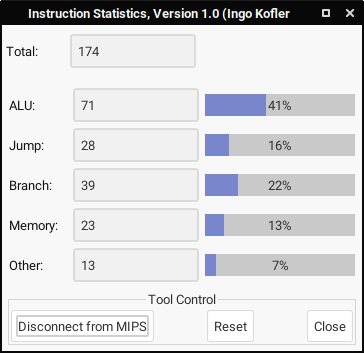
\includegraphics[width=242px]{questao2_stats}
	\\\footnotesize Fonte: Mars Instruction Statistic Tool
\end{figure}

\pagebreak

\begin{flushleft}
	\nocite{*}
	\bibliography{TP1}
	\vfill
	O histórico do desenvolvimento desse trabalho se encontra online em:\\ \url{https://github.com/Durfan/ufsj-aoc1-tp1}.
\end{flushleft}

\end{document}
